
\documentclass[12pt,twoside,dvipsnames,letterpaper]{memoir}
%% GENERAL ADD ONS %%%%%%%%%%%%%%%%%%%%%%%%%%%%%%%%%%%%%%%%%%%%%%%%%%%%%%%%%%%%

\usepackage[dvipsnames]{xcolor}  %% Must come before Tikz etc.
\usepackage[many]{tcolorbox}
\usepackage{dcounter}
\usepackage{enumerate}
\usepackage{graphicx}
\usepackage[
    hyperindex=true,
    colorlinks=true,
    linkcolor=teal,
    citecolor=ForestGreen]{hyperref}
\usepackage{float}     %% given captions to listings and types.
\usepackage{caption}
\usepackage{subcaption}
% \usepackage{aeguill}  %% IF NEEDED INCLUDE IN Content.tex near top
\usepackage[light]{kpfonts} % Nice Adobe Font
\usepackage{pifont} % \xmark
    \newcommand{\cmark}{\ding{51}}%
    \newcommand{\xmark}{\ding{55}}%

%% TIKZ %%%%%%%%%%%%%%%%%%%%%%%%%%%%%%%%%%%%%%%%%%%%%%%%%%%%%%%%%%%%%%%%%%%%%%%
\usepackage{tikz}
\usepackage{tikz-cd}
    \usetikzlibrary{positioning,arrows,backgrounds}
%%%%%%%%%%%%%%%%%%%%%%%%%%%%%%%%%%%%%%%%%%%%%%%%%%%%%%%%%%%%%%%%%%%%%%%%%%%%%%%

%% MATH %%%%%%%%%%%%%%%%%%%%%%%%%%%%%%%%%%%%%%%%%%%%%%%%%%%%%%%%%%%%%%%%%%%%%%%

\usepackage{amsmath,amsthm,amssymb}

\newcommand{\bigforall}{\mbox{\Large $\mathsurround0pt\forall$}}
\newcommand{\bigexists}{\mbox{\Large $\mathsurround0pt\exists$}}


\usepackage{bussproofs}  %% proof diagrams
\usepackage{wasysym} % \Leftcircle
\usepackage{mathtools}  % left/right harpoons
% \usepackage{lscape}  %% Landscape pages.
% \usepackage{longtable}  %% tables that span 2 pages

%%%%%%%%%%%%%%%%%%%%%%%%%%%%%%%%%%%%%%%%%%%%%%%%%%%%%%%%%%%%%%%%%%%%%%%%%%%%%%%
% \usepackage{zref-abspos} % Used to know where digress/focus starts/ends

%% STYLE CHAPTERS %%%%%%%%%%%%%%%%%%%%%%%%%%%%%%%%%%%%%%%%%%%%%%%%%%%%%%%%%%%%%
\makechapterstyle{invhangnum}{%
  \setlength\beforechapskip{0pt}%
  \renewcommand*\chapterheadstart{\vspace{\beforechapskip}}%
  \setlength\afterchapskip{2\onelineskip plus .2\onelineskip minus 0.2\onelineskip}%  
  \renewcommand\chaptitlefont{\Huge\bfseries}
  \setlength\midchapskip{-\baselineskip}%
  \renewcommand\chapnumfont{\Huge\bfseries}
  \renewcommand*{\printchaptername}{}
  \renewcommand*{\chapternamenum}{}
  \renewcommand*{\printchapternum}{%
      \raisebox{\dimexpr\midchapskip+\baselineskip\relax}[0pt][0pt]{%
        \makebox[0pt][l]{%
        \makebox[\dimexpr\textwidth+4em\relax][l]{%
          \parbox[t]{\textwidth}{\mbox{}}%
          \parbox[t]{4em}{\hfill\chapnumfont \thechapter}}}}}%
  \renewcommand*{\printchaptertitle}[1]{%
    \raisebox{\dimexpr\midchapskip+\baselineskip\relax}[0pt][0pt]{%
      \parbox[t]{\textwidth}{\raggedright\chaptitlefont ##1}}}%
}
\chapterstyle{invhangnum}
\newlength{\digresslen}
% \chapterstyle{hangnum}
% \hangsecnum

    \usepackage{eso-pic}   %% Used to add gray strip to side of pages.
    %%%%%%%%% Digression margins.
    % \newenvironment{}{}{}
    \newcommand{\digresshere}[1]{
        % \newdimen\digheight
        % \setbox0=\vbox{#1}
        % \digheight=\ht0 \advance\digheight by \dp0
        % \zsavepos{#1-digress}
        % \write\mywrite{#1: \zposy{#1-digress}}%
        % \AddToShipoutPictureBG{%
        % \AtPageLowerLeft{%
        
            % \ifodd\value{page}
            % \hspace*{\dimexpr\paperwidth-3em}%
            % \fi
            % \settoheight{\digresslen}{\vbox{#1}}
        \marginpar{\hspace{\marginparwidth}\textcolor{black!25}{\rule{3em}{1in}}}%
        % }%
        % }%
        % \newcommand{\focus}{\ClearShipoutPictureBG}
    }

    \newcommand{\digress}{
        % \zsavepos{#1-digress}
        % \write\mywrite{#1: \zposy{#1-digress}}%
    \AddToShipoutPictureBG{%
        \AtPageLowerLeft{%
        %\raisebox{.25\paperheight}{%
            \ifodd\value{page}
            \hspace*{\dimexpr\paperwidth-3em}%
            \fi
            \textcolor{black!25}{\rule{3em}{\paperheight}}%
        %}%
        }%
        }
    }
    \newcommand{\focus}{\ClearShipoutPictureBG}
    \newcommand{\codemargin}[1]{
        \marginpar{
            \colorbox{black!25}{
                \parbox{0.9\marginparwidth}{
                    {\small \textsf{#1}}
                }
            }
        }
    }
    %% TOC Formatting
    % Indentation of numbers
    \setlength{\cftsectionindent}{2em}      % default 1.5em

    % Distance between numbers and titles
    \setlength{\cftpartnumwidth}{2.25em}      % default 1.5em
    \setlength{\cftchapternumwidth}{2em}      % default 1.5em
    \setlength{\cftsectionnumwidth}{3em}      % default 2.3em





\usepackage{imakeidx}
    \makeindex
    \indexsetup{headers={Index}{Index}} % Left/Right headers for the index

    \newcommand{\term}[1]{\emph{#1}}%\index{#1}}
%%%%%%%%%%%%%%%%%%%%%%%%%%%%%%%%%%%%%%%%%%%%%%%%%%%%%%%%%%%%%%%%%%%%%%%%%%%%%%%

%% TITLE PAGE %%%%%%%%%%%%%%%%%%%%%%%%%%%%%%%%%%%%%%%%%%%%%%%%%%%%%%%%%%%%%%%%%
\usepackage{epigraph}
\usepackage{titling}
\usepackage{bookman}
    \renewcommand\epigraphflush{flushright}
    \renewcommand\epigraphsize{\normalsize}
    \setlength\epigraphwidth{0.7\textwidth}

    % CSU Green 92, 18, 94, 61
    \definecolor{titlepagecolor}{cmyk}{.92,.18,.94,.61}
    % CSU Gold 11, 6, 64, 13
    \definecolor{titlepagecolor2}{cmyk}{.11,.06,.64,.13}
    %\definecolor{titlepagecolor}{cmyk}{1,.60,0,.40}

    \DeclareFixedFont{\titlefont}{T1}{ppl}{b}{it}{0.5in}
    % The following code is borrowed from: https://tex.stackexchange.com/a/86310/10898

    %%% STOLEN FROM 
    %%%% https://tex.stackexchange.com/questions/85904/showcase-of-beautiful-title-page-done-in-tex
    \newcommand\titlepagedecoration{%
    \begin{tikzpicture}[remember picture,overlay,shorten >= -10pt]

    \coordinate (aux1) at ([yshift=-15pt]current page.north east);
    \coordinate (aux2) at ([yshift=-410pt]current page.north east);
    \coordinate (aux3) at ([xshift=-4.5cm]current page.north east);
    \coordinate (aux4) at ([yshift=-150pt]current page.north east);

    \begin{scope}[titlepagecolor!40,line width=12pt,rounded corners=12pt]
    \draw
    (aux1) -- coordinate (a)
    ++(225:5) --
    ++(-45:5.1) coordinate (b);
    \draw[shorten <= -10pt]
    (aux3) --
    (a) --
    (aux1);
    \draw[opacity=0.6,titlepagecolor2,shorten <= -10pt]
    (b) --
    ++(225:2.2) --
    ++(-45:2.2);
    \end{scope}
    \draw[titlepagecolor,line width=8pt,rounded corners=8pt,shorten <= -10pt]
    (aux4) --
    ++(225:0.8) --
    ++(-45:0.8);
    \begin{scope}[titlepagecolor!70,line width=6pt,rounded corners=8pt]
    \draw[shorten <= -10pt]
    (aux2) --
    ++(225:3) coordinate[pos=0.45] (c) --
    ++(-45:3.1);
    \draw
    (aux2) --
    (c) --
    ++(135:2.5) --
    ++(45:2.5) --
    ++(-45:2.5) coordinate[pos=0.3] (d);   
    \draw 
    (d) -- +(45:1);
    \end{scope}
    \end{tikzpicture}%
    }


%%%%%%%%%%%%%%%%%%%%%%%%%%%%%%%%%%%%%%%%%%%%%%%%%%%%%%%%%%%%%%%%%%%%%%%%%%%%%%%

%% STYLE POPOUTS %%%%%%%%%%%%%%%%%%%%%%%%%%%%%%%%%%%%%%%%%%%%%%%%%%%%%%%%%%%%%%

\usepackage{tcolorbox}
    \newenvironment{guide}[1]{
        \medskip
        \begin{center}
        \begin{minipage}[t]{0.95\linewidth} %{\dimexpr0.33\textwidth-2\fboxrule-2\fboxsep\relax}
            \begin{tcolorbox}[colback=gray!5,colframe=green!40!black,title=#1]
    }{
            \end{tcolorbox}
        \end{minipage}
        \end{center}
        \medskip
    }%
    \newenvironment{mywarning}[1] {
        \medskip
        \begin{center}
        \begin{minipage}[t]{0.95\linewidth} %{\dimexpr0.33\textwidth-2\fboxrule-2\fboxsep\relax}
            \begin{tcolorbox}[colback=gray!5,colframe=red!40!black,title=#1]
    }{
            \end{tcolorbox}
        \end{minipage}
        \end{center}
        \medskip
    }%
    \newenvironment{open}{
        \medskip
        \begin{center}
        \begin{minipage}[t]{0.95\linewidth} %{\dimexpr0.33\textwidth-2\fboxrule-2\fboxsep\relax}
            \begin{tcolorbox}[colback=gray!5,colframe=blue!40!black,title=Open Problem]
    }{
            \end{tcolorbox}
        \end{minipage}
        \end{center}
        \medskip
    }%
%%%%%%%%%%%%%%%%%%%%%%%%%%%%%%%%%%%%%%%%%%%%%%%%%%%%%%%%%%%%%%%%%%%%%%%%%%%%%%%





%% FONTS %%%%%%%%%%%%%%%%%%%%%%%%%%%%%%%%%%%%%%%%%%%%%%%%%%%%%%%%%%%%%%%%%%%%%%
% \usepackage{fontspec}
% \usepackage[T1]{fontenc}
% \usepackage{kpfonts}
% \usepackage[T1]{fontenc}

%% AUTHOR INDEX %%%%%%%%%%%%%%%%%%%%%%%%%%%%%%%%%%%%%%%%%%%%%%%%%%%%%%%%%%%%%%%

\newcommand{\Church}{\index{Church, Alonzo (1903--1995)}}
\newcommand{\Codd}{\index{Codd, Edgar F. (1923--2003)}}
\newcommand{\Coquand}{\index{Coquand, Thierry (1961--)}}
\newcommand{\Curry}{\index{Curry, Haskell (1900--1982)}}
\newcommand{\Frege}{\index{Frege, Gottlob (1884--1925)}}
\newcommand{\Hamilton}{\index{Hamilton, Sir William Rowan (1805--1865)}}
\newcommand{\Hopper}{\index{Hopper, Grace (1906--1992)}}
\newcommand{\Leibniz}{\index{Leibniz, Gottfried (1646--1716)}}
\newcommand{\MartinLof}{\index{Martin-Lof@Martin-L\"of, Per (1942--)}}
\newcommand{\Russell}{\index{Russell, Bertrand (1872--1970)}}
\newcommand{\Tarski}{\index{Tarski, Alfred (1901--1983)}}
\newcommand{\Turing}{\index{Turing, Alan (1912--1954)}}
\newcommand{\Whitehead}{\index{Whithead, Alfred North (1861--1947)}}
\newcommand{\ZF}{\index{Zermelo, Ernst (1871--1953)}\index{Fraenkel, Abraham (1891--1965)}}




%% FINAL SETTINGS %%%%%%%%%%%%%%%%%%%%%%%%%%%%%%%%%%%%%%%%%%%%%%%%%%%%%%%%%%%%%
\numberwithin{figure}{chapter}
\numberwithin{table}{chapter}

%% EDITING MARKS %%%%%%%%%%%%%%%%%%%%%%%%%%%%%%%%%%%%%%%%%%%%%%%%%%%%%%%%%%%%%%
\usepackage[draft]{pdfcomment}
\usepackage{xparse}
    \DeclareDocumentCommand \EDITmargin { o m } {
        \IfNoValueTF {#1} {
            \pdfmargincomment[icon=Note]{#2}
        }{
            \pdfmargincomment[icon=NOte,author=#1]{#2}
        }
    }
    \DeclareDocumentCommand \EDITcomment { o m } {
        \IfNoValueTF {#1} {
            \pdfcomment[color=Blue!20]{#2}
        }{
            \pdfcomment[color=Blue!20,author=#1]{#2}
        }
    }
    \DeclareDocumentCommand \EDITalt { o m m } {
        \IfNoValueTF {#1} {
            \pdfmarkupcomment[markup=StrikeOut]{#2}{#3}
        }{
            \pdfmarkupcomment[markup=StrikeOut,icon=key, author=#1]{#2}{#3}
        }
    }
    \DeclareDocumentCommand \EDITtypo { o m o } {
        \IfNoValueTF {#3} {
            \pdfmarkupcomment[markup=Squiggly,author=#1]{#2}{}
        }{
            \pdfmarkupcomment[markup=Squiggly,author=#1]{#2}{#3}
        }
    }
    \DeclareDocumentCommand \EDIThighlight { o m m } {
        % \IfNoValueTF {#3} {
        %     \pdfmarkupcomment[markup=Highlight,author=#1,color=blue!20]{#2}{}
        % }{
            \pdfmarkupcomment[markup=Highlight,author=#1,color=blue!20]{#2}{#3}
        % }
    }


    
%%%%%%%%%%%%%%%%%%%%%%%%%%%%%%%%%%%%%%%%%%%%%%%%%%%%%%%%%%%%
%% Theorems
\usepackage{thmtools}
\declaretheoremstyle[
    shaded={
        rulecolor=black!30,
        rulewidth=1pt,    
        bgcolor=white
    }
]{thm}
\declaretheorem[numberwithin=chapter, style=thm]{theorem}
\declaretheorem[sibling=theorem, style=thm]{lemma}
\declaretheorem[sibling=theorem, style=thm]{proposition}
\declaretheorem[sibling=theorem, style=thm]{corollary}


\declaretheoremstyle[
    shaded={
        rulecolor=purple!30,
        rulewidth=1pt,    
        bgcolor=white
    }
]{eg}
% \declaretheorem[sibling=theorem, style=eg]{ex}
\declaretheorem[sibling=theorem, style=eg]{example}

\declaretheoremstyle[
    shaded={
        rulecolor=teal!20,
        rulewidth=1pt,    
        bgcolor=white
    }
]{def}
\declaretheorem[sibling=theorem, style=def]{definition}

\declaretheoremstyle[
    shaded={
        rulecolor=ForestGreen,
        rulewidth=1pt,    
        bgcolor=white
    }
]{rem}
\declaretheorem[sibling=theorem, style=rem]{remark}

\declaretheorem[sibling=theorem, name=Engineering Note, style=rem]{implremark}
\declaretheorem[sibling=theorem, name=Historical Remark, style=rem]{histremark}

%-----------------------------------------------------
%       Standard theorem like environments.
%-----------------------------------------------------
%% \theoremstyle{plain} %% This is the default
\numberwithin{equation}{chapter}
%\newtheorem{theorem}[equation]{Theorem}
%\newtheorem*{theorem*}{Theorem}
%\newtheorem{lemma}[equation]{Lemma}
%\newtheorem{proposition}[equation]{Proposition}
\newtheorem{prob}{}[chapter]

%\newtheorem{lem}[equation]{Lemma}
%\newtheorem{corollary}[equation]{Corollary}
%\newtheorem*{coro*}{Corollary}
\newtheorem{quest}[equation]{Question}

\theoremstyle{remark}


\theoremstyle{definition}
%\newtheorem{definition}[equation]{Definition}
%\newtheorem{ex}{Example}[equation]
% \newtheorem*{remark*}{Remark}
% \newtheorem{remark}[equation]{Remark}
% \newtheorem{progrem}[equation]{Programing Remark}
% \newtheorem{histrem}[equation]{Historical Remark}



%%%%%%%%%%%%%%%%%%%%%%%%%%%%%%%%%%%%%%%%%%%%%%%%%%%%%%%%%%%

\newcommand{\plusplus}{{\tiny ++}}

\newcommand{\tsspace}{\mathsf{space}~}
\newcommand{\tsaxes}{\mathsf{axes}~}
\newcommand{\tsframe}{\mathsf{frame}~}
\newcommand{\tsbase}{\mathsf{base}~}
\newcommand{\tsinterp}{\mathsf{interp.}~}


\newcommand{\NamedTensorSpace}[6]{
\begin{array}{lllll}
    #1 & \defeq \mathsf{TensorSpace}\big(
        &\tsspace & #2,\\
&        &\tsaxes & #3,\\
&        &\tsframe & #4,\\
&        &\tsbase & #5,\\            
&        &\tsinterp & #6 ~~~\big)        
    \end{array}
}
\newcommand{\TensorSpace}[5]{
\begin{array}{lll}
\mathsf{TensorSpace}\big(
        &\tsspace & #1,\\
        &\tsaxes & #2,\\
        &\tsframe & #3,\\
        &\tsbase & #4,\\            
        &\tsinterp & #5 ~~~\big)        
    \end{array}
}
\newcommand{\InlineTensorSpace}[5]{
$\mathsf{TensorSpace}($ 
    $\tsspace #1$, 
    $\tsaxes #2$,
    $\tsframe #3$,
    $\tsbase #4$,
    $\tsinterp #5$)
}
%\usepackage[dvipsnames]{xcolor}
%\usetikzlibrary{external}
%\tikzexternalize[prefix=figures/] % activate and define figures/ as cache folder

\newcommand{\elastic}{-\dimexpr\pgfmatrixcolumnsep+0.6em\relax}

\tikzset{pics/.cd,
opencube/.style args={#1/#2/#3}{code={
\coordinate (O) at (0,0,0);
\coordinate (A) at (0,#2,0);
\coordinate (B) at (0,#2,#3);
\coordinate (C) at (0,0,#3);
\coordinate (D) at (#1,0,0);
\coordinate (E) at (#1,#2,0);
\coordinate (F) at (#1,#2,#3);
\coordinate (G) at (#1,0,#3);
%% Background
\draw[black,dotted] (O) -- (A);
\draw[black,dotted] (O) -- (C);
\draw[black,dotted] (O) -- (D);
% Forground
\draw[black,dashed] (A) -- (E) -- (F) -- (B) -- cycle;
\draw[black,dashed] (E) -- (D) -- (G) -- (C) -- (B);
\draw[black,dashed] (F) -- (G);

%\draw[black,dashed, blue] (O) -- (A) -- (E) -- (D) -- cycle;
%\draw[black,dashed] (O) -- (A) -- (B) -- (C) -- cycle;
%\draw[black,dashed] (D) -- (E) -- (F) -- (G) -- cycle;
%\draw[black,dashed] (C) -- (B) -- (F) -- (G) -- cycle;
%\draw[black,dashed] (A) -- (B) -- (F) -- (E) -- cycle;

}}}

%%%%%%%%%%%%%%%%%%%%%%%%%%%%%%%%%%%%%%%%%%%%%%%%%%%%%%%%%%%%%%%%%%%%%%%%%%%
%% Print a shaded cube of row/column/width  / contents
%%%%%%%%%%%%%%%%%%%%%%%%%%%%%%%%%%%%%%%%%%%%%%%%%%%%%%%%%%%%%%%%%%%%%%%%%%%
\tikzset{pics/.cd,
linecube/.style args={#1/#2/#3/#4}{code={
\coordinate (OO) at (0,0,0);
\coordinate (AA) at (0,#2,0);
\coordinate (BB) at (0,#2,#3);
\coordinate (CC) at (0,0,#3);
\coordinate (DD) at (#1,0,0);
\coordinate (EE) at (#1,#2,0);
\coordinate (FF) at (#1,#2,#3);
\coordinate (GG) at (#1,0,#3);
%% Background
\draw[black,dashed] (OO) -- (AA);
\draw[black,dashed] (OO) -- (CC);
\draw[black,dashed] (OO) -- (DD);

\node at (0.5*#1,0.5*#2,0.5*#3) {#4};

% Foreground
\draw[black] (AA) -- (EE) -- (FF) -- (BB) -- cycle;
\draw[black] (EE) -- (DD) -- (GG) -- (CC) -- (BB);
\draw[black] (FF) -- (GG);

%\draw[black,dashed, blue] (O) -- (A) -- (E) -- (D) -- cycle;
%\draw[black,dashed] (O) -- (A) -- (B) -- (C) -- cycle;
%\draw[black,dashed] (D) -- (E) -- (F) -- (G) -- cycle;
%\draw[black,dashed] (C) -- (B) -- (F) -- (G) -- cycle;
%\draw[black,dashed] (A) -- (B) -- (F) -- (E) -- cycle;

}}}

%%%%%%%%%%%%%%%%%%%%%%%%%%%%%%%%%%%%%%%%%%%%%%%%%%%%%%%%%%%%%%%%%%%%%%%%%%%
%% Print a shaded cube of row/column/width / color / contents
%%%%%%%%%%%%%%%%%%%%%%%%%%%%%%%%%%%%%%%%%%%%%%%%%%%%%%%%%%%%%%%%%%%%%%%%%%%
\tikzset{pics/.cd,
shadedcube/.style args={#1/#2/#3/#4/#5}{code={
\coordinate (O) at (0,0,0);
\coordinate (A) at (0,#2,0);
\coordinate (B) at (0,#2,#3);
\coordinate (C) at (0,0,#3);
\coordinate (D) at (#1,0,0);
\coordinate (E) at (#1,#2,0);
\coordinate (F) at (#1,#2,#3);
\coordinate (G) at (#1,0,#3);
\draw[black,fill=#4!80] (O) -- (C) -- (G) -- (D) -- cycle;
\draw[black,fill=#4!30] (O) -- (A) -- (E) -- (D) -- cycle;
\draw[black,fill=#4!10] (O) -- (A) -- (B) -- (C) -- cycle;
\draw[black,fill=#4!20,opacity=0.8] (D) -- (E) -- (F) -- (G) -- cycle;
\draw[black,fill=#4!20,opacity=0.6] (C) -- (B) -- (F) -- (G) -- cycle;
\draw[black,fill=#4!20,opacity=0.8] (A) -- (B) -- (F) -- (E) -- cycle;
\node at (0.5*#1,0.5*#2,0.5*#3) {#5};
}}}


%%%%%%%%%%%%%%%%%%%%%%%%%%%%%%%%%%%%%%%%%%%%%%%%%%%%%%%%%%%%%%%%%%%%%%%%%%%
%% Print a cube of subcubes, row/column/width / subrows / subcols / subwid / color
%%%%%%%%%%%%%%%%%%%%%%%%%%%%%%%%%%%%%%%%%%%%%%%%%%%%%%%%%%%%%%%%%%%%%%%%%%%
\tikzset{pics/.cd,
gridcube/.style args={#1/#2/#3/#4/#5/#6/#7}{code={
\coordinate (O) at (0,0,0);
\coordinate (A) at (0,#2,0);
\coordinate (B) at (0,#2,#3);
\coordinate (C) at (0,0,#3);
\coordinate (D) at (#1,0,0);
\coordinate (E) at (#1,#2,0);
\coordinate (F) at (#1,#2,#3);
\coordinate (G) at (#1,0,#3);

% Foreground
\draw[fill=#7!20] (A) -- (E) -- (F) -- (B) -- cycle;
\draw[fill=#7!40] (E) -- (F) -- (G) -- (D) -- cycle;
\draw[fill=#7!30] (B) -- (F) -- (G) -- (C) -- cycle;
%\draw[black] (E) -- (D) -- (G) -- (C) -- (B);
%\draw[black] (F) -- (G);

% lines
\foreach \ll in {1,...,#4} {
    \draw[black] (#1/#4*\ll,#2,0) -- (#1/#4*\ll,#2,#3) -- (#1/#4*\ll,0,#3);
}
\foreach \ll in {1,...,#5} {
    \draw[black] (0,#2/#5*\ll,#3) -- (#1, #2/#5*\ll,#3) -- (#1,#2/#5*\ll,0);
}
\foreach \ll in {1,...,#6} {
    \draw[black] (0,#2,#3/#6*\ll) -- (#1,#2,#3/#6*\ll) -- (#1,0,#3/#6*\ll);
}

}}}

\tikzset{pics/.cd,
%%% y/z/color/label
lwing/.style args={#1/#2/#3/#4}{code={
\coordinate (O) at ( 0, 0, 0);
\coordinate (A) at ( 0, 0,#2);
\coordinate (B) at ( 0,#1,#2);
\coordinate (C) at ( 0,#1, 0);
\draw[black,fill=#3] (O) -- (A) -- (B) -- (C) -- cycle;
\node at (0,0.5*#1,0.5*#2) {#4};
}}}

%%% FLAT COLOR RECTANGLE WITH ENTRY
\tikzset{pics/.cd,
mwing/.style args={#1/#2/#3/#4/#5}{code={
\coordinate (O) at ( 0, 0, 0);
\coordinate (A) at (#1, 0, 0);
\coordinate (B) at (#1,#2, 0);
\coordinate (C) at ( 0,#2, 0);
\draw[black,fill=#5!20] (O) -- (A) -- (B) -- (C) -- cycle;
\node at (0.5*#1,0.5*#2,0) {#4};
}}}

\tikzset{
    pics/.cd,
    % width/lenght/xticks/yticks/bgcolor
    matrix/.style args={#1/#2/#3/#4/#5}{
        code={
            \coordinate (O) at ( 0, 0, 0);
            \coordinate (A) at (#1, 0, 0);
            \coordinate (B) at (#1,#2, 0);
            \coordinate (C) at ( 0,#2, 0);
            \fill[color=#5] (O) -- (A) -- (B) -- (C) -- cycle;
            \foreach \x in {0,...,#3} {
                \draw[black] (#1/#3*\x,0,0) -- ++(0,#2,0);
            }
            \foreach \y in {0,...,#4} {
                \draw[black] (0,#2/#4*\y,0) -- ++(#1,0,0);
            }
        }
    }
}

\tikzset{
    pics/.cd,
    % width/lenght/xticks/yticks/bgcolor
    rmatrix/.style args={#1/#2/#3/#4/#5}{
        code={
            \coordinate (O) at ( 0, 0, 0);
            \coordinate (A) at (#1, 0, 0);
            \coordinate (B) at (#1, 0, #2);
            \coordinate (C) at ( 0, 0, #2);
            \fill[color=#5] (O) -- (A) -- (B) -- (C) -- cycle;
            \foreach \x in {0,...,#3} {
                \draw[black] (#1/#3*\x,0,0) -- ++(0,0,#2);
            }
            \foreach \z in {0,...,#4} {
                \draw[black] (0,0,0#2/#4*\z) -- ++(#1,0,0);
            }
        }
    }
}

\tikzset{
    pics/.cd,
    % width/lenght/xticks/yticks/bgcolor
    lmatrix/.style args={#1/#2/#3/#4/#5}{
        code={
            \coordinate (O) at ( 0, 0, 0);
            \coordinate (A) at ( 0, 0,#2);
            \coordinate (B) at ( 0,#1,#2);
            \coordinate (C) at ( 0,#1, 0);
            \fill[color=#5] (O) -- (A) -- (B) -- (C) -- cycle;
            \foreach \z in {0,...,#4} {
                \draw[black] (0,0,#2/#4*\z) -- ++(0,#1,0);
            }
            \foreach \y in {0,...,#3} {
                \draw[black] (0,#1/#3*\y,0) -- ++(0,0,#2);
            }
        }
    }
}

% \tikzset{pics/.cd,
% mwing/.style args={#1/#2/#3/#4}{code={
% \coordinate (O) at ( 0, 0, 0);
% \coordinate (A) at (#1, 0, 0);
% \coordinate (B) at (#1,#2, 0);
% \coordinate (C) at ( 0,#2, 0);
% \draw[black,fill=green!20] (O) -- (A) -- (B) -- (C) -- cycle;
% \node at (0.5*#1,0.5*#2,0) {#4};
% }}}

\tikzset{pics/.cd,
%% x/z/color/label
rwing/.style args={#1/#2/#3/#4}{code={
\coordinate (O) at ( 0, 0, 0);
\coordinate (A) at (#1, 0, 0);
\coordinate (B) at (#1, 0,#2);
\coordinate (C) at ( 0, 0,#2);
\draw[black,fill=#3] (O) -- (A) -- (B) -- (C) -- cycle;
\node at (0.5*#1,0,0.5*#2) {#4};
}}}

\tikzset{pics/.cd,
    abacus2/.style args={#1/#2}{
        code={
            \draw[red] (0,0) -- (1.5,0);
            \draw[red] (0,0.25) -- (1.5,0.25);
            \foreach \u in {1,...,#1} {
                \filldraw[red] (0.1*\u,0) circle (1pt);
            }
            \foreach \u in {1,...,#2} {
                \filldraw[red] (0.1*\u,0.25) circle (1pt);
            }
        }
    } 
}

\tikzset{pics/.cd,
    abacus3/.style args={#1/#2/#3/#4}{
        code={
            \draw[#4] (0,0) -- (1.5,0);
            \draw[#4] (0,0.25) -- (1.5,0.25);
            \draw[#4] (0,0.5) -- (1.5,0.5);
            \foreach \u in {1,...,#1} {
                \filldraw[#4] (0.1*\u,0) circle (1pt);
            }
            \foreach \u in {1,...,#2} {
                \filldraw[#4] (0.1*\u,0.25) circle (1pt);
            }
            \foreach \u in {1,...,#3} {
                \filldraw[#4] (0.1*\u,0.5) circle (1pt);
            }
        }
    } 
}

\usepackage{xparse}
\DeclareDocumentCommand \next { m } {\acute{#1}} %{\dot{#1}}
\DeclareDocumentCommand \nnext { m }  {\text{\H{#1}}} %{\ddot{#1}} %{\H{#1}}

%\usepackage{ulem} % for \uline
%\renewcommand{\ULdepth}{1pt}
\newcommand{\fullsupp}[1]{\underline{#1}}
\newcommand{\rrto}{\substack{\rightarrow\\[-1em] \rightarrow}}
\newcommand{\llto}{\substack{\leftarrow\\[-1em] \leftarrow}}

%% Homotopism arrows.
\newcommand{\ddd}{\downarrow\downarrow\downarrow}
\newcommand{\ddu}{\downarrow\downarrow\uparrow}
\newcommand{\dde}{\downarrow\downarrow\|}
\newcommand{\dud}{\downarrow\uparrow\downarrow}
\newcommand{\duu}{\downarrow\uparrow\uparrow}
\newcommand{\due}{\downarrow\uparrow\|}
\newcommand{\ded}{\downarrow\|\downarrow}
\newcommand{\deu}{\downarrow\|\uparrow}
\newcommand{\dee}{\downarrow\|\|}
%%
\newcommand{\udd}{\uparrow\downarrow\downarrow}
\newcommand{\udu}{\uparrow\downarrow\uparrow}
\newcommand{\ude}{\uparrow\downarrow\|}
\newcommand{\uud}{\uparrow\uparrow\downarrow}
\newcommand{\uuu}{\uparrow\uparrow\uparrow}
\newcommand{\uue}{\uparrow\uparrow\|}
\newcommand{\ued}{\uparrow\|\downarrow}
\newcommand{\ueu}{\uparrow\|\uparrow}
\newcommand{\uee}{\uparrow\|\|}
%%
\newcommand{\edd}{\|\downarrow\downarrow}
\newcommand{\edu}{\|\downarrow\uparrow}
\newcommand{\ede}{\|\downarrow\|}
\newcommand{\eud}{\|\uparrow\downarrow}
\newcommand{\euu}{\|\uparrow\uparrow}
\newcommand{\eue}{\|\uparrow\|}
\newcommand{\eed}{\|\|\downarrow}
\newcommand{\eeu}{\|\|\uparrow}
\newcommand{\eee}{\|\|\|}

\newcommand{\cev}[1]{\reflectbox{\ensuremath{\vec{\reflectbox{\ensuremath{#1}}}}}}

%% Making a Minecraft Walrus := that doesn't use circular dots
%% so that it doesn't clash with : for types.
\usepackage{scalerel}  %\hstretch
\newcommand{\defeq}{\mathrel{\hstretch{.13}{=}\hspace{.2ex}{=}}}%\coloneqq} %\newcommand{\defeq}{\overset{\mathrm{def}}{=\joinrel=}}
\newcommand{\betaeq}{\rightleftharpoons}

%--Shortcuts--

%%%%%%%%%%%%%%%%%%%%%%%%%%%%%%%%%%%%%%%

\DeclareMathOperator{\Hol}{Hol}
\DeclareMathOperator{\chr}{char }
\DeclareMathOperator{\trace}{tr~}
\DeclareMathOperator{\rad}{rad }
\DeclareMathOperator{\torrad}{torrad }
\DeclareMathOperator{\Fun}{Fun }
\DeclareMathOperator{\Hom}{hom }
\DeclareMathOperator{\End}{End}
\DeclareMathOperator{\Nil}{Nil }
\DeclareMathOperator{\Ric}{Rich }
\DeclareMathOperator{\Scal}{Scal }
\DeclareMathOperator{\Sym}{Sym }
\DeclareMathOperator{\Alt}{Alt }
\DeclareMathOperator{\Her}{Her }
\DeclareMathOperator{\Adj}{Adj }
\DeclareMathOperator{\Der}{Der }
\DeclareMathOperator{\Spin}{Spin }
\DeclareMathOperator{\JSpin}{JSpin }
\DeclareMathOperator{\GL}{GL}
\DeclareMathOperator{\PGL}{PGL}
\DeclareMathOperator{\SL}{SL}
\DeclareMathOperator{\Sp}{Sp}
\DeclareMathOperator{\GO}{GO}
\DeclareMathOperator{\GU}{GU}
\DeclareMathOperator{\GF}{GF}
\DeclareMathOperator{\Gal}{Gal }
\DeclareMathOperator{\Gr}{Gr}
\DeclareMathOperator{\Nuc}{Nuc}
\DeclareMathOperator{\Cen}{Cen}
\DeclareMathOperator{\Id}{Id}
\DeclareMathOperator{\Null}{Null}
% Lie algebras.
\DeclareMathOperator{\gl}{\mathfrak{gl}}
%\DeclareMathOperator{\sl}{\mathfrak{sl}}
%\DeclareMathOperator{\so}{\mathfrak{so}}
%\DeclareMathOperator{\sp}{\mathfrak{sp}}
\DeclareMathOperator{\Inn}{Inn}
\DeclareMathOperator{\Aut}{Aut}
\DeclareMathOperator{\Inv}{Inv}
\DeclareMathOperator{\Isom}{Isom}
\DeclareMathOperator{\Str}{Str}
\DeclareMathOperator{\Stab}{Stab}
\DeclareMathOperator{\memb}{memb}
\DeclareMathOperator{\Cent}{Cen}
\DeclareMathOperator{\img}{img }
\DeclareMathOperator{\Res}{Res }
\DeclareMathOperator{\Ann}{Ann }
\DeclareMathOperator{\Prob}{Pr}
\DeclareMathOperator{\rank}{rank }
\DeclareMathOperator{\Diag}{Diag }
\DeclareMathOperator{\gr}{gr}
\DeclareMathOperator{\lcm}{lcm}
\DeclareMathOperator{\disc}{disc}
\DeclareMathOperator{\Out}{Out}
\DeclareMathOperator{\out}{out}
\DeclareMathOperator{\supp}{supp}
\DeclareMathOperator{\im}{Im}
\DeclareMathOperator{\Type}{Type}
\DeclareMathOperator{\Span}{Span}
\DeclareMathOperator{\Pres}{Pres}
%\DeclareMathOperator{\MyFree}{F}
\newcommand{\MyFree}{\mathbf{F}}
\newcommand{\Free}[2][]{\MyFree_{#1}^{#2}}
\DeclareMathOperator{\Lin}{Lin}
\DeclareMathOperator{\Rel}{Rel}
\DeclareMathOperator{\inj}{inj}
\DeclareMathOperator{\sur}{sur}
\newcommand{\refl}{\mathsf{refl}}

\newcommand{\Comm}[1]{{\mathsf{Comm}\textrm{-}{#1}}}
\newcommand{\Set}{{\mathsf{Set}}}

\DeclareMathOperator{\ad}{ad}

\newcommand{\R}{\mathbb{R}}
\newcommand{\M}{\mathbb{M}}
\newcommand{\cond}[2]{\overset{#1}{{_{#1}#2}_{#1}}}

\newcommand{\Bi}{\mathsf{Bi} }
\newcommand{\Grp}{\mathsf{Grp} }

\newcommand{\lt}[1]{{#1}^{\Lsh}}
\newcommand{\rt}[1]{{#1}^{\Rsh}}
\newcommand{\lr}[1]{{#1}^{\Lsh\Rsh}}
\newcommand{\ct}[1]{{#1}^{\uparrow}}
\newcommand{\perpsum}{\perp} %% \obot is prefered and uses mathabx
\newcommand{\op}{\circ}

\newcommand{\CC}{\mathcal{C}}
\newcommand{\LL}[1]{\mathcal{L}_{#1}}
\newcommand{\RR}[1]{\mathcal{R}_{#1}}
\newcommand{\MM}[1]{\mathcal{M}_{#1}}
\newcommand{\LMR}{\mathcal{LMR}}
\newcommand{\sprod}{\Pi\,}

%======== CORRESPONDENCE ==============
%\newcommand{\Ten}[2]{\mathscr{N}(#1,#2)}
%\newcommand{\Id}[2]{\mathscr{I}(#1,#2)}
%\newcommand{\Op}[2]{\mathscr{Z}(#1,#2)}

\DeclareMathOperator{\ID}{Id}
\DeclareMathOperator{\id}{id}


%\usepackage{ifsym} % \TriangleRight
\newcommand{\trip}[3]{{_{#2}^{#1}} #3}

\newcommand{\rversor}{\,\reflectbox{\ensuremath{\oslash}}\,}%\obackslash}
\newcommand{\lversor}{\oslash}

\newcommand{\bm}{*}
\newcommand{\bmto}{\rightarrowtail}
\newcommand{\TSU}{U_0\oslash\cdots\oslash U_{\vav}}


%  TUPLES===============
%\usepackage[T1]{fontenc}% http://ctan.org/pkg/fontenc
\newcommand{\mm}[1]{\langle #1\rangle}
\newcommand{\la}{\langle}
\newcommand{\ra}{\rangle}

%% IF NEEDED within Content.tex uncomment '% \usepackage{aeguill}'
%% Position in preamble matters so don't move!
% \newcommand{\lga}{\textnormal{\guillemotleft}}
% \newcommand{\rga}{\textnormal{\guillemotright}}

\usepackage{stmaryrd}
\newcommand{\llparen}{\Leftcircle}
\newcommand{\rrparen}{\Rightcircle}
\makeatletter
\newsavebox{\@brx}
\newcommand{\lla}[1][]{\savebox{\@brx}{\(\m@th{#1\langle}\)}%
  \mathopen{\copy\@brx\kern-0.5\wd\@brx\usebox{\@brx}}}
\newcommand{\rra}[1][]{\savebox{\@brx}{\(\m@th{#1\rangle}\)}%
  \mathclose{\copy\@brx\kern-0.5\wd\@brx\usebox{\@brx}}}
\makeatother

\newcommand{\bbinom}[2]{\begin{bmatrix} #1\\ #2 \end{bmatrix}}

%\newcommand{\comp}[1]{\bar{#1}}
%\newcommand{\widecomp}[1]{\overline{#1}}
\newcommand{\lsa}{\sphericalangle}
\newcommand{\rsa}{\reflectbox{\ensuremath{\sphericalangle}}}
\newcommand{\llb}{\llbracket}
\newcommand{\rrb}{\rrbracket}
\newcommand{\llp}{\llparenthesis}
\newcommand{\rrp}{\rrparenthesis}

%\newcommand{\TSat}[3]{#1_{\vDash #2(#3)}}
%\newcommand{\PSat}[3]{{_{#1\vDash}{#2}}_{#3}}
%\newcommand{\OpSat}[3]{{_{#1\vDash #2}#3}}

\newcommand{\bra}[1]{\la #1\,|}
\newcommand{\ket}[1]{|\,#1\ra}
\newcommand{\braket}[2]{\la #1\,|\,#2\ra}
\newcommand{\1}{\mathbbm{1}}

\newcommand{\range}[1]{[#1]}

\newcommand{\zrange}[1]{\llbracket #1\rrbracket}



\newenvironment{bsmat}{
    \left[\begin{smallmatrix}
}{
    \end{smallmatrix}\right]
}

\usepackage{relsize}  %\mathlarger
\newcommand{\Forall}{\mathop{\mathlarger{\mathlarger{\forall}}}}
\newcommand{\Exists}{\mathop{\mathlarger{\mathlarger{\exists}}}}

\newcommand{\from}{\leftarrow}


%%%%%%%%%%%%%%%%%%%%%%%%%%%%%%%%%%

\newcommand{\form}[1]{\mathtt{F}_{#1}}
\newcommand{\intro}[1]{\mathtt{I}_{#1}}
\newcommand{\comp}[1]{\mathtt{C}_{#1}}
\newcommand{\acomp}[1]{\approx\mathtt{C}_{#1}}
\newcommand{\elim}[1]{\mathtt{E}_{#1}}

\newcommand{\CombS}[1]{\mathbb{S}_{#1}}
\newcommand{\CombK}[1]{\mathbb{K}_{#1}}
\newcommand{\CombI}{\mathbb{I}}


\newcommand{\lstintable}[2][]{\lstinline[#1]{#2}}
\newcommand{\at}{\,@\,}



\usepackage{cjhebrew}
    \DeclareFontFamily{U}{rcjhbltx}{}
    \DeclareFontShape{U}{rcjhbltx}{m}{n}{<->rcjhbltx}{}
    \DeclareSymbolFont{hebrewletters}{U}{rcjhbltx}{m}{n}

    % remove the definitions from amssymb
    \let\aleph\relax\let\beth\relax
    \let\gimel\relax\let\daleth\relax

    \DeclareMathSymbol{\aleph}{\mathord}{hebrewletters}{39}
    \DeclareMathSymbol{\beth}{\mathord}{hebrewletters}{98}\let\bet\beth
    \DeclareMathSymbol{\gimel}{\mathord}{hebrewletters}{103}
    \DeclareMathSymbol{\daleth}{\mathord}{hebrewletters}{100}\let\dalet\daleth

    \DeclareMathSymbol{\lamed}{\mathord}{hebrewletters}{108}
    \DeclareMathSymbol{\mem}{\mathord}{hebrewletters}{109}\let\mim\mem
    \DeclareMathSymbol{\ayin}{\mathord}{hebrewletters}{96}
    \DeclareMathSymbol{\tsadi}{\mathord}{hebrewletters}{118}
    \DeclareMathSymbol{\qof}{\mathord}{hebrewletters}{114}
    \DeclareMathSymbol{\shin}{\mathord}{hebrewletters}{152}
    \DeclareMathSymbol{\waw}{\mathord}{hebrewletters}{119}
    \DeclareMathSymbol{\vavv}{\mathord}{hebrewletters}{119}
    \DeclareMathOperator{\vav}{{{\ensuremath{\vavv}\,}}}


    

%% Program Listings %%%%%%%%%%%%%%%%%%%%%%%%%%%%%%%%%%%%%%%%%%%%%%%%%%%%%%%%%%%

% \usepackage[many]{tcolorbox}

\usepackage{listings}
% \usepackage[many]{tcolorbox}




%% FLOAT %%%%%%%%%%%%%%%%%%%%%%%%%%%%%%%%%%%%%%%%%%%%%%%%%%%%%%%%%%%%%%%%%%%%%%
\newfloat{lstfloat}{htbp}{lop}
\floatname{lstfloat}{Listing}
\numberwithin{lstfloat}{chapter}

\floatstyle{ruled}
\newfloat{typefloat}{htbp}{lop}
\floatname{typefloat}{Type}
\numberwithin{typefloat}{chapter}
%%%%%%%%%%%%%%%%%%%%%%%%%%%%%%%%%%%%%%%%%%%%%%%%%%%%%%%%%%%%%%%%%%%%%%%%%%%%%%%

%% Hanna %%%%%%%%%%%%%%%%%%%%%%%%%%%%%%%%%%%%%%%%%%%%%%%%%%%%%%%%%%%%%%%%%%%%%%
\definecolor{dkgreen}{rgb}{0,0.6,0}
\definecolor{gray}{rgb}{0.5,0.5,0.5}
\definecolor{mauve}{rgb}{0.58,0,0.82}
% \lstdefinelanguage{Hanna}{
%     morekeywords={def,:,=, abstract, interface, class, trait, private, for, while, if, then, else, yield  },
%     sensitive=false, % keywords are not case-sensitive
%     morecomment=[l]{//}, % l is for line comment
%     morecomment=[s]{/*}{*/}, % s is for start and end delimiter
%     morestring=[b]" % defines that strings are enclosed in double quotes
% } 

%% Sava %%%%%%%%%%%%%%%%%%%%%%%%%%%%%%%%%%%%%%%%%%%%%%%%%%%%%%%%%%%%%%%%%%%%%%
%% a hybrid C/Java/Scala styled procedural dialect
\lstdefinelanguage{Sava}{
    morekeywords={
        def,
        :,
        =, 
        constructor,
        using,
        require,
        class, 
        alias, 
        abstract, 
        seal, 
        trait, 
        void, 
        until, 
        repeat, 
        return, 
        extends, 
        ext, 
        override, 
        case, 
        new, 
        for, 
        private, 
        postulate,
        while, 
        if, 
        then, 
        else, 
        yield, 
        import, 
        from, 
        abstract, 
        in, 
        print, 
        match,
        implicit,
        with,
        ->
    },
    sensitive=false, % keywords are not case-sensitive
    morecomment=[l]{//}, % l is for line comment
    morecomment=[s]{/*}{*/}, % s is for start and end delimiter
    morestring=[b]" % defines that strings are enclosed in double quotes
    backgroundcolor=\color{WhiteSmoke},
    %frame=tb,
} %

%% Hidris %%%%%%%%%%%%%%%%%%%%%%%%%%%%%%%%%%%%%%%%%%%%%%%%%%%%%%%%%%%%%%%%%%%%%%
%% a hybrid Lisp/Haskell/Idirs functional dialect
\lstdefinelanguage{Hidris}{
    morekeywords={
        data, 
        lambda, 
        class, 
        import, 
        type, 
        :, 
        alias, 
        instance, 
        where, 
        let, 
        from, 
        match, 
        with,
        postulate
    },
    sensitive=false, % keywords are not case-sensitive
    morecomment=[l]{---}, % l is for line comment
    morestring=[b]" % defines that strings are enclosed in double quotes
    backgroundcolor=\color{lightblue},
} %
%%%%%%%%%%%%%%%%%%%%%%%%%%%%%%%%%%%%%%%%%%%%%%%%%%%%%%%%%%%%%%%%%%%%%%%%%%%%%%%

%% Sava %%%%%%%%%%%%%%%%%%%%%%%%%%%%%%%%%%%%%%%%%%%%%%%%%%%%%%%%%%%%%%%%%%%%%%
%% a hybrid relational database Query Language like SQL
\lstdefinelanguage{PseudoQL}{
    morekeywords={
        CREATE,
        BEGIN,
        END,
        TYPE,
        OBJECT,
        RETURN, 
        BODY,
        MEMBER,
        FUNCTION,
        AS,
        IS,
    },
    sensitive=true, % keywords are not case-sensitive
    morecomment=[l]{--}, % l is for line comment
    morecomment=[s]{/*}{*/}, % s is for start and end delimiter
    morestring=[b]" % defines that strings are enclosed in double quotes
    backgroundcolor=\color{WhiteSmoke},
    %frame=tb,
} %

%% Main  %%%%%%%%%%%%%%%%%%%%%%%%%%%%%%%%%%%%%%%%%%%%%%%%%%%%%%%%%%%%%%%%%%%%%%
%% a generic REPL style
\lstdefinestyle{main}{
% frame=trbl,
  aboveskip=3mm,
  belowskip=3mm,
  showstringspaces=false,
  %columns=flexible,
  basicstyle={\small\ttfamily},
  numbers=none,
  numberstyle=\tiny\color{gray},
  keywordstyle=\color{blue},
  commentstyle=\color{dkgreen},
  stringstyle=\color{mauve},
  breaklines=true,
  breakatwhitespace=true,
  tabsize=2
}

%% Table  %%%%%%%%%%%%%%%%%%%%%%%%%%%%%%%%%%%%%%%%%%%%%%%%%%%%%%%%%%%%%%%%%%%%%%
%% use in listings within tables
\lstdefinestyle{tablestyle}{
    frame=none,
  aboveskip=3mm,
  belowskip=3mm,
  showstringspaces=false,
  %columns=flexible,
  basicstyle={\small\ttfamily},
  numbers=none,
  numberstyle=\tiny\color{gray},
  keywordstyle=\color{blue},
  commentstyle=\color{dkgreen},
  stringstyle=\color{mauve},
  breaklines=true,
  breakatwhitespace=true,
  tabsize=2
}

\lstset{style=main}

% Notebook styled listings.=======================
\tcbuselibrary{listings}


% the space reserved between for the ``In'' numbers and the code
\newlength\inwd
\setlength\inwd{1.3cm}
\newcounter{notebookcounter}


\newfloat{lstfloat}{htbp}{lop}
\floatname{lstfloat}{Listing}
\numberwithin{lstfloat}{section}

\colorlet{inputcolor}{blue!50!black}
\colorlet{outputcolor}{red!50!black}

\lstdefinelanguage{genericnotebookin}{
    morekeywords={print, def, return},
    morecomment=[l]{//},
    basicstyle=\footnotesize\ttfamily,
    keywordstyle=\color{green!40!black}\bfseries,
    commentstyle=\color{purple!40!black}\itshape,
}

\lstdefinelanguage{genericnotebookout}{
    morekeywords={:,Type},
    morecomment=[l]{//},
    basicstyle=\footnotesize\ttfamily,
    keywordstyle=\bfseries\color{green!40!black},
    commentstyle=\itshape\color{purple!40!black},
}

\newtcblisting{notebookin}[1][\thenotebookcounter]{
  enlarge left by=\inwd,
  width=\linewidth-\inwd,
  enhanced,
  boxrule=0.4pt,
  colback=ForestGreen!15,
  listing only,
  top=0pt,
  bottom=0pt,
  overlay={
    \node[
      anchor=north east,
      text width=\inwd,
      font=\footnotesize\ttfamily\color{inputcolor},
      inner ysep=2mm,
      inner xsep=0pt,
      outer sep=0pt
      ] 
      at (frame.north west)
      {\stepcounter{notebookcounter}{\small In [#1]}};
  }
  listing engine=listing,
  listing options={
    aboveskip=1pt,
    belowskip=1pt,
    language=genericnotebookin,
    showstringspaces=false,
    breaklines=true,
  },
}
\newtcblisting{notebookout}[1][\thenotebookcounter]{
  enlarge left by=\inwd,
  width=\linewidth-\inwd,
  enhanced,
  boxrule=0.1pt,% 0.4pt,
  colback=White,
  listing only,
  top=0pt,
  bottom=0pt,
  overlay={
    \node[
      anchor=north east,
      text width=\inwd,
      font=\footnotesize\ttfamily\color{outputcolor},
      inner ysep=2mm,
      inner xsep=0pt,
      outer sep=0pt
      ] 
      at (frame.north west)
      {Out\,[#1]};
  }
  listing engine=listing,
  listing options={
    aboveskip=1pt,
    belowskip=1pt,
    language=genericnotebookout,
    showstringspaces=false,
  },
}

%=================================================

\tikzset{Rightarrow/.style={double equal sign distance,>={Implies},->},
triple/.style={-,preaction={draw,Rightarrow}},
quadruple/.style={preaction={draw,Rightarrow,shorten >=0pt},shorten >=1pt,-,double,double
distance=0.2pt}}

\floatstyle{ruled}
\newfloat{typefloat}{htbp}{lop}
\floatname{typefloat}{Type}






\author{James B. Wilson}
\date{\today}
\begin{document}


\section*{Kernels}

\subsection{Kernels in Set language}
Given $\Omega$-modules $V$ and $W$ and a linear map $\varphi:V\to W$, 
\[
    \ker \varphi=\{v\in V\mid \varphi(v)=0\}.
\]
This definition is concise because it's meaning
is outsourced to the concept of a set. Let us see how 
far this gets us. 
For example, suppose we are given $\varphi$ by a matrix 
\begin{align*}
    \Phi & = 
    \begin{bmatrix}
        1 & 1 & 0 & 3\\
        1 & 0 & 2 & 5\\
        1 & 1 & 0 & 3
    \end{bmatrix}
\end{align*}
So what is in $\ker\varphi$?  The set 
offers no answer.

% Thus any properties of $\ker\varphi$ will need to be 
% developed from within that system. There are two complications. 
% First most persons, and a positive proportion of mathematicians,
% cannot state the rules for sets.  Second, the full 
% spectrum of set properties is well-beyond what can be computed 
% or proved consistent.  In fact, even the fundamental axioms 
% are not a finite list but must instead involve axioms schema
% and ramification.  There is nothing wrong with using these 
% properties, unless you don't know what any of that means.
% But we are not motivated to explain laws and logic of all 
% sets, we simply want to understand and use kernels.  So 
% what follows are alternative definitions that can each 
% be described in a handful of precise rules and are amenable 
% to computing.

\subsection{Kernels in Computer Algebra Systems}
We can begin by inputting a linear mapping (as a matrix) into a computer algebra system.
\begin{notebookin}
Phi = [ 1 1 1; 1 0 1; 0 2 0; 3 5 3 ]
print Phi
\end{notebookin}
\begin{notebookout}[\thenotebookcounter]
[ 1 1 0 3 ]
[ 1 0 2 5 ]
[ 1 1 0 3 ]
\end{notebookout}
Research shows humans make 3-6 errors per hour, no matter 
what the task is.  Why waste any of 
them on miscalculating?  Let us ask a computer for the kernel.
\begin{notebookin}
K = Kernel(Phi)
print K
\end{notebookin}
\begin{notebookout}[\thenotebookcounter]
[ -2 -5 ]
[  2  2 ]
[  1  0 ]
[  0  1 ]
\end{notebookout}
This may be a surprise.  This is a matrix, not a 
set.  Why?



\subsection{Kernels in Diagram language}
To decode the difference between the set-wise concept of a kernel 
and what a program provides, we start with an alternative definition of kernels 
using diagrams and focussed on what it means to put data into the kernel
and to get data out of the kernel.

We start with a linear map, and so that gives us our first diagram.
It is introduced with $\forall$ because it applies to \emph{all} linear maps.
We should also indicate somewhere that that context is modules, which 
we do once at the start by writing ${_{\Omega} \mathsf{Mod}}$.  Often 
we authors skip that step letting context be know implicitly.
\begin{center}
    \begin{tikzpicture}
        %% For All
        \node[outer sep=5pt] (form) at (0,0) 
        {\begin{tikzcd}[background color=black!15,column sep=tiny]
            W & \phantom{J} & V \arrow[ll,"\varphi"{above}]
        \end{tikzcd}};
    
        \node (all) at (form.north west) {$\forall$};
        \draw[thick] (all.south) -- (form.south west);

        \node (text) at (form.north) {${_{\Omega}\mathsf{Mod}}$};
    \end{tikzpicture}       
\end{center}

Kernels exist for every linear map and will appear as a new structure denoted 
$\ker\varphi$.  This on its own would have no relation to $\varphi$ in the diagram, so we draw out that relationship by adding new arrows, new 
linear functions that is.  One arrow is 
just $0$, and the second $\iota$ is injective.  

The $0$ arrow should be explained a bit, it just means $0(x)=x$.  
This is an uneventful step but its role will unfold as necessary because it 
will offer the constraint to the equations that follow.  Without it there would 
be no equations and thus no solutions.  Note, some authors prefer to take 
two steps for zero functions pausing to pass through the zero module 
$\{0\}$.  Somewhat confusingly that space is also written as $0$. Get used to it but prepared to explain your own missuses of 0 should anyone ask you.
So instead of writing $0:A\to B$ some authors will write a sequence of arrows 
$A\to 0\to B$.

The real star is the arrow denoted by $\iota$ which feeds into the arrow $\varphi$.  Lining up the arrows 
indicates we can compose 
these two functions $\varphi\circ \iota$.  This should equal the other 
arrow reaching the same point, namely $0$.  So $\varphi\circ \iota=0$,
or rather $\varphi(\iota(k))=0$ for $k\in \ker\varphi$.  We say the 
diagram \emph{commutes} and we indicate this by shading the background.
\begin{center}
    \begin{tikzpicture}
    %% There exists
    \node[outer sep=5pt, fill=black!15] (form) at (4,0) 
    {\begin{tikzcd}[
        background color=black!15,
        column sep=tiny
        ]
        W & & V\arrow[ll,"\varphi"{above}]\\
            & \ker\varphi\arrow[lu,"0"{below}]\arrow[ur,hook,"\iota"{below}]
    \end{tikzcd}};

    \node (exists) at (form.north west) {$\exists$};
    \draw[thick] (exists.south) -- (form.south west);
\end{tikzpicture}  
\end{center}
The $\iota$ in this diagram is a new linear map, and so it could be 
given by a matrix.  In the example given earlier, the matrix 
$\Phi$ produced a kernel function $\iota$ whose matrix was the matrix
that our computer produced.  So through our new lens of kernels the 
computer output is correct, we should get a matrix not a set.

Unfortunately we cannot stop here even though we have the promised kernel.
This is because many spaces $K$ and functions $\kappa:K\to V$ could play the role of
$\ker\varphi$ as shown in the above diagram without actually being the 
kernel we have in mind.  For example, $K=\{0\}$ certainly would do the same 
but the matrix $\Phi$ given earlier we expect a different answer.  So this cannot
be a complete understanding of kernels.  We need $\ker\varphi$ to be ``as big as
possible''.  Even saying that we find a puzzle because what would it mean 
for a function to be ``as big as possible''.  To resolve this let us 
add to our diagram an other data and functions that can match what we already 
know about kernels.
\begin{center}
    \begin{tikzpicture}
    %% For All constraints
    \node[outer sep=5pt, fill=black!15] (constraint) at (8,0) 
    {\begin{tikzcd}[background color=black!15,column sep=tiny]
        W & & V\arrow[ll,"\varphi"{above}]\\
         & \ker\varphi\arrow[lu,"0"{below}]\arrow[ur,hook,"\iota"{below}]\\
         & K \arrow[uul,bend left,"0"{below}]\arrow[uur, hook, bend right, "\kappa"{below}]
    \end{tikzcd}};

    \node (all2) at (constraint.north west) {$\forall$};
    \draw[thick] (all2.south) -- (constraint.south west);
        
    \end{tikzpicture}
\end{center}
The quantifier $\forall$ here now ranges over $\kappa:K\to V$ so we are 
setting ourselves up to compare how our chosen $\ker\varphi$ compares to 
any other possible solution.

The conclusion you might have guessed is that if our solution should be 
at least as capable as any other, and to diagram that we simply need that 
every alternative solution can be mapped into our own $\ker \varphi$.  So there
exists a unique new arrow $K\to \ker\varphi$ transforming any competitor data 
into data of our own type, as shown below.
\begin{center}
\begin{tikzpicture}
    %% exist unique
    \node[outer sep=5pt, fill=black!15] (universal) at (12,0) 
    {\begin{tikzcd}[background color=black!15,column sep=tiny]
        W & & V\arrow[ll,"\varphi"{above}]\\
         & \ker\varphi\arrow[lu,"0"{below}]\arrow[ur,hook,"\iota"{below}]\\
         & K \arrow[uul,bend left,"0"{below}]\arrow[uur, hook, bend right, "\kappa"{below}]\arrow[u]
    \end{tikzcd}};

    \node (unique) at (universal.north west) {$\exists !$};
    \draw[thick] (unique.south) -- (universal.south west);
    
\end{tikzpicture}    
\end{center}

Like frames in a graphic novel, these four diagrams should be read 
as a timeline, see Figure~\ref{fig:kernel-diag}.  
\begin{figure}[!htbp]
\begin{center}
    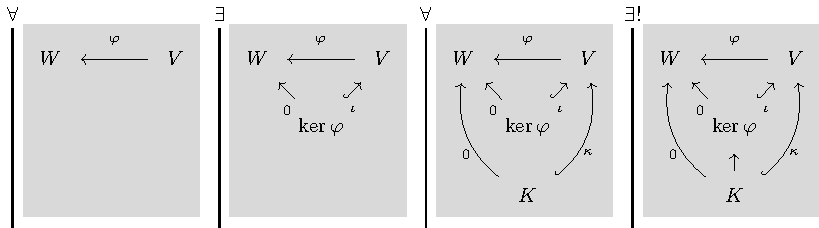
\includegraphics[width=\textwidth]{kernel-graphic.pdf}
\end{center}
\caption{The diagram description of kernels.}
\label{fig:kernel-diag}
\end{figure}

This pattern of 
``$\forall \exists\forall\exists!$'' will be repeated many times in similar 
constructions.  In fact the longer we work with logical puzzles we will 
find the steady use of the pattern 
\begin{align*}
    \Pi_n & \equiv \overbrace{\forall \exists\cdots \forall \exists}^n
    & 
    \Sigma_n & \equiv \overbrace{\exists\forall\cdots \exists\forall}^n.
\end{align*}
These organizations of logical sentences was introduced by Kleene and 
Mostowski and is known today as the \emph{Arithmetical Hierarchy}.
Programmers who ask how hard it is to prove statements in that Hierarchy 
will find they have invented the \emph{Polynomial-time Hierarchy}.
So it is worth getting comfortable with the meaning, but we warned 
that answering questions in these hierarchies could earn you a million Euro 
prize and your name in the newspaper.  One of the leading questions 
is this tower may one day collapse, meaning that you only need to go 
to some fixed value of $n$ before you know everything.

\subsection{Kernels in Typed language}

The diagram language clarifies how kernels can be thought of as functions and 
functions that have a maximal quality.  Yet, programs do not think in pictures, 
we do.  So we need to translate the same ideas to a syntax we can turn into a 
program.  Here is how.

First the question depends on $\Omega$-modules $V$ and $W$ and a linear map $\varphi:V\to W$ 
known first from context, denoted $\mathsf{ctx}$ or $\Gamma$.  Using the notation 
$P\vdash Q$ to say ``$P$ leads to $Q$'', also denoted $\frac{P}{Q}$, then we can 
state this as forming the kernel under a list of assumed knowledge.
\begin{gather}
    \tag{$\form{\ker}$}
    \frac{
        \mathsf{ctx} \vdash V,W:{_{\Omega} \mathsf{Mod}}\qquad
        \varphi:\mathsf{Lin}_{\Omega}(V,W)
    }{
        \mathsf{ctx}\vdash \ker\varphi:\mathsf{Type}
    }
\end{gather}
The label $\form{\ker}$ stands for \emph{formation}.  Programs write this in
many different ways usually by introducing some keywords like ``import''
and ``use X from Y'.  To introduce a new type of data a keyword such as ``class''
or ``type'' is used.  For example, the following pseudo-code reflects the 
content of $(\form{\ker})$ but in a dialect similar to several modern 
procedural programming 
languages such as C++ and Java.
\begin{lstlisting}[language=Sava]
using V,W:Mod[Omega], Phi:Lin[V,W] from ctx
class Ker[Phi] {...}
\end{lstlisting}
For those using functional programming languages like OCaml or Haskell the following syntax offers 
as similar translation.
\begin{lstlisting}[language=Hidris]
import V,W:Mod Omega, Phi:Lin V W from ctx
type Ker Phi
\end{lstlisting}



\begin{lstfloat}[!htbp]
\begin{lstlisting}[language=Sava]
// Procedural style code
class Ker[Phi](k:K,kappa:K->V) where (Phi(kappa(k)) == 0)
// usage 
Phi = ...; k = ...; kappa = ...;
x = new Ker[Phi](k,kappa)
\end{lstlisting}
\begin{lstlisting}[language=Hidris]
--- Functional style code
type Ker Phi
null: (k:K)-> (kappa:K->V)-> (Phi kappa k == 0)-> Ker Phi
--- usage 
Phi= ...; k= ...; kappa= ...;
x= null Phi k kappa --- system checks Phi kappa k == 0
\end{lstlisting}    
\caption{An introduction of data to a kernel.}
\label{lst:kernel-intro}
\end{lstfloat}
    
Next the diagram above captured the high-level movement of that data without 
ever considering the actual data.  The programs will certainly need these 
data.  The premise from the diagram is that any data $k:K$ which is found to 
have $\kappa(k):V$ where $\varphi(\kappa(j))=0$ (see the diagrams above) must 
produce data in $\ker\varphi$.
Any such data $k:K$ is meant to produce data in the kernel, because the 
kernel is the largest such structure.  So we include such a rule.
\begin{gather}
    \tag{$\intro{\ker}$}
    \frac{
        k:K\qquad \kappa:K\to V\qquad pf:\varphi(\kappa(k))=_W 0
    }{
        \mathsf{null}(\kappa(k)):\ker\varphi
    }
\end{gather}
The $\intro{\ker}$ here is for \emph{introduction} because data is 
being introduced of the desired type.  
Most readers will not be prepared for the meaning of symbols like:
\[
    pf:\varphi(\kappa(k))=_W 0
\] 
Programmers however are uniquely well-positioned to guess the meaning. We want
some data $pf$ that has the type $\varphi(\kappa(k))=0$ in $W$. Said another
way, we need someone to provide a proof of that equality. In programs this can
be done by several tricks most common are what are known as \emph{guards} or
\emph{rails}.  These are a type of documentation added to a program to let the
programming language enforce that data is used in restricted ways.  In this
case, no one can introduce a term in the kernel without proof. In code this can
be captured in a number of ways, Listing~\ref{lst:kernel-intro} is one option.

% The introduction of data of some kind is known 
% to programmers as a \emph{constructor} and many languages make special 
% rules to specify constructors.  For uniformity and simplicity we here 
% use `def' to introduce all service functions to a data type and name 
% the function to match the notation used in the mathematical formalism.
% But any real program will adapt the vocabulary and style to fit with 
% conventions.


Now it is time to use data in the kernel.  It is clear how this should 
proceed, anything in the kernel can be mapped to $0$ in $W$ or to a 
value in $V$ which will map to $0$ under $\varphi$.  The rules are therefore 
as follows.    
\begin{gather}
    \tag{$\elim{\ker}$}
    \frac{
        x:\ker\phi
    }{
        0:W
    }\qquad
    \frac{
        x:\ker\phi
    }{
        \iota(x):V
    }
\end{gather}
The name $\elim{\ker}$ stands for \emph{elimination} as we are eliminating 
the kernel type to get to new types.
In code this might be done as shown in the code fragment Listing~\ref{lst:kernel-elim}.
\begin{lstfloat}[!htbp]
\begin{lstlisting}[language=Sava]
// Procedural style code
class Ker[Phi](k:K,kappa:K->V) where (Phi(kappa(k))== 0){
    def iota:V = ...
    def zero:W = ...
}
// usage 
x = new Ker[Phi](k,kappa)
v = x.iota
\end{lstlisting}
\begin{lstlisting}[language=Hidris]
--- Functional style code
iota: Ker Phi -> V
...
zero: Ker Phi -> W
...
--- usage 
x= null Phi k kappa --- system checks Phi kappa k == 0
v = iota x
\end{lstlisting}    
\caption{Using of data of kernel type.}
\label{lst:kernel-elim}
\end{lstfloat}

Finally we need to do some computing somewhere and we learn 
what to compute by inspecting the condition of ``commutative diagrams''.
\begin{gather}
    \tag{$\comp{\ker}$}
    \frac{
        k:K\qquad \kappa:K\to V\qquad pf:\varphi(\kappa(j))=_W 0
    }{
        \iota(x) \defeq \kappa(k)
    }
\end{gather}
All together this comes together in software in many different ways 
each designed around different techniques to improve how we read and 
execute code.  Listing~\ref{lst:kernel-comp} provides some of the options.
\begin{lstfloat}[!htbp]
\begin{lstlisting}[language=Sava]
// Procedural style code
class Ker[Phi](k:K,kappa:K->V) where (Phi(kappa(k))== 0){
    def iota:V = kappa(k)
    def zero:W = 0
}
// usage 
x = new Ker[Phi](k,kappa)
v = x.iota
\end{lstlisting}
\begin{lstlisting}[language=Hidris]
--- Functional style code
iota: Ker Phi -> V
iota x = kappa k where x = null k kappa
zero: Ker Phi -> W
zero x = 0
--- usage 
x= null Phi k kappa --- system checks Phi kappa k == 0
v = iota x
\end{lstlisting}    
\caption{Using of data of kernel type.}
\label{lst:kernel-elim}
\end{lstfloat}
\begin{lstfloat}
\begin{lstlisting}[language=Sava]
using V,W:Mod[Omega], Phi:Lin[V,W] from ctx
class Ker[Phi] {
    private v:V

    def null(j:J, kappa:J->V, 
        require Phi(kappa(j)) == 0) {
        v = kappa(j)    
    }
    def iota:V = v
    def zero:W = 0
}
\end{lstlisting}
\caption{A complete data type for kernels}    
\end{lstfloat}


\subsection{Computing a kernel}
Algorithms appearing in China around 2000 years
ago appear to depict a version of computing kernels.
A thousand years later in Irag and Iran the inventers of 
algebra were solving systems of linear equations which 
would necessitate the ability to solve kernels as well.
In the 1800's Gauss's many contributions to math included 
a systematic algorithm to solve for kernels.  Once you 
have learned Gauss's method it becomes impossible to think 
of any other likely solution.  For that reason the historic 
examples are usually conjectured to be the same algorithm.

Let us consider a matrix in which a subset of the columns 
are an identity matrix.  That is, up to possibly permuting 
the columns the matrix has the form
\begin{align*}
    \begin{bmatrix}
        I_r & M \\ 
        0 & 0 
    \end{bmatrix}\in \Delta^{m\times n}
\end{align*}
Then an answer would be written down with formula 
requiring no computation:
\begin{align*}
    \begin{bmatrix}
        I_r & M \\ 
        0 & 0 
    \end{bmatrix}
    \begin{bmatrix}
        -M^{\dagger}  \\ 
        I_{n-r} 
    \end{bmatrix}
    & = 
    \begin{bmatrix}
        0\\
        0
    \end{bmatrix}
\end{align*}


\begin{align*}
    \Phi & = 
    \begin{bmatrix}
        1 & 1 & 0 & 3\\
        0 & -1 & -2 & -2\\
        0 & 0 & 0 & 0
    \end{bmatrix}
\end{align*}





\subsection{Uniqueness questions}

\end{document}